% id: 144-32
% book: 100발100중 3-1 기말 · 01 3-1 기말(이차방정식·이차함수·부록)
% section: 고난도 기출문제
% figure: crop:fig-144-32.png
% answer: ③
% answer_source: 답지(빠른정답)
% variant_level: 0 (원본 전사)
% 이 파일은 build.mjs 가 items.json 에서 만든다. 고칠 때는 items.json 을 고친다.
\smash{\raisebox{1.5mm}{\dmkichul{100발100중 3-1 기말 144쪽 32번}}}
\noindent\begin{minipage}[t]{0.58\linewidth}\vspace{0pt}\raggedright 그림과 같이 이차함수 $y=x^2$의 그래프 위의 점~$\pt{P}_1(1{,}\mkern3mu 1)$을 잡고, $\overline{\pt{OP}_1}$을 잇는다. 또, 점~$\pt{P}_1$을 지나고 $x$축에 평행한 직선을 그어 포물선과 만나는 다른 한 점을 $\pt{P}_2$라 하고, 점~$\pt{P}_2$를 지나고 직선 $\pt{OP}_1$에 평행한 직선을 그어 포물선과 만나는 다른 한 점을 $\pt{P}_3$이라고 한다. 이와 같은 방법으로 교점과 직선을 계속 그려나갈 때, $\triangle\pt{P}_3\pt{P}_4\pt{P}_5$의 넓이는?\end{minipage}\hfill\begin{minipage}[t]{0.4\linewidth}\vspace{0pt}\centering 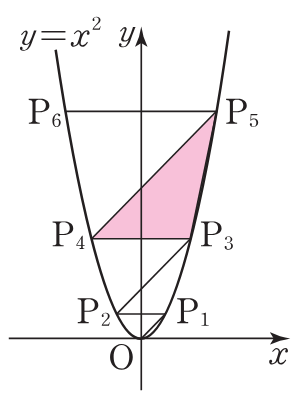
\includegraphics[width=71.6pt]{figures/fig-144-32.png}\end{minipage}\par
\begin{choices32}{$6$}{$8$}{$10$}{$12$}{$14$}\end{choices32}
